\subsection{UC4 - Interazione con lo staff}\label{usecase:4}
%diagramma dei casi d'uso 4
\begin{figure}[H]
  \centering
  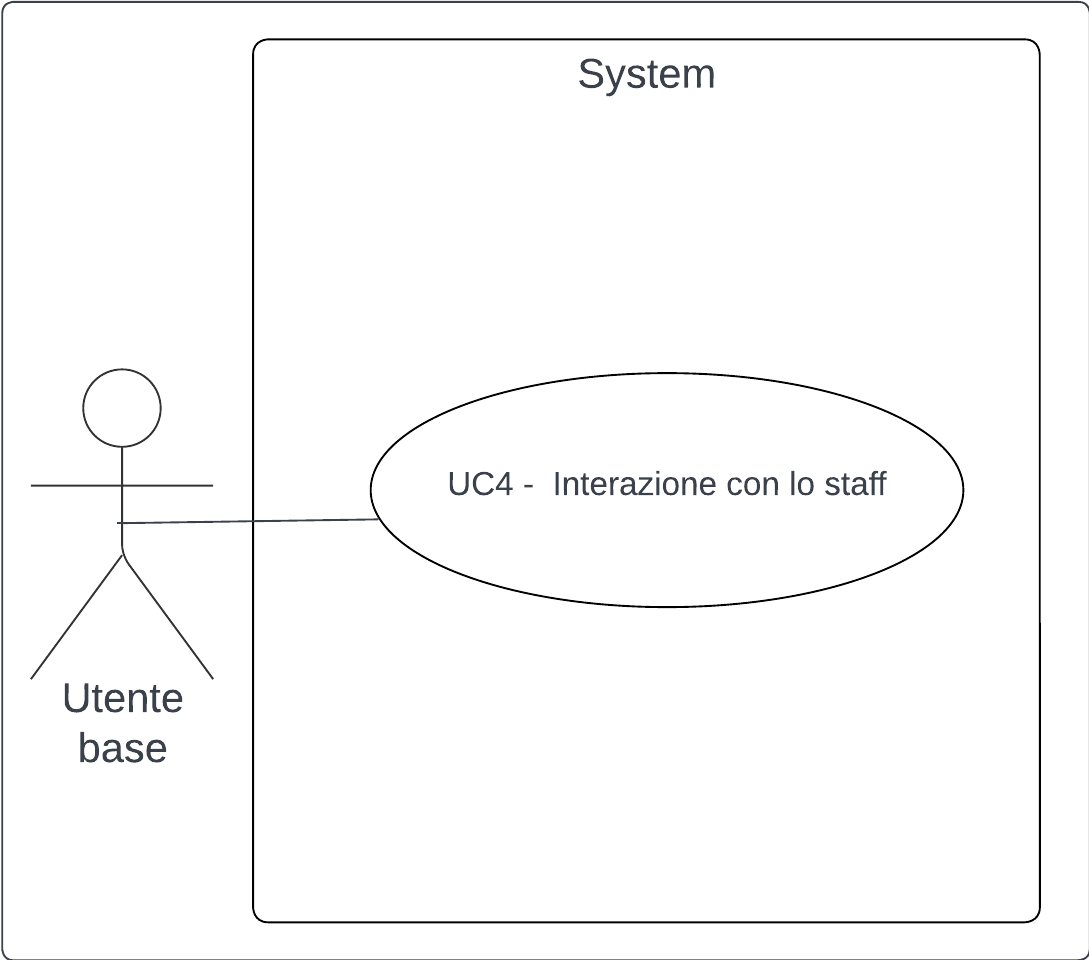
\includegraphics[width=0.9\textwidth]{ucd/UCD4.png}
  \caption{Interazione con lo staff}
\end{figure}
\textbf{Attori}:
\begin{itemize}
    \item Utente base.
\end{itemize}
\textbf{Precondizioni}:
\begin{itemize}
    \item L'utente è connesso al $\textit{Sistema}_G$.
     \item La chat è stata avviata.
\end{itemize}
\textbf{Postcondizioni}:
\begin{itemize}
    \item L'utente ha comunicato con l'amministratore del ristorante.
\end{itemize}
\textbf{Scenario principale}:
\begin{enumerate}
    \item L'utente seleziona un ristorante desiderato;
    \item Il $\textit{sistema}_G$ crea una chat bidirezionale;
    \item L'utente può comunicare con l'amministratore del ristorante:
    \begin{itemize}
        \item L'utente può scrivere del testo e inviarlo (\nameref{usecase:4_1});
        \item L'utente visualizza l'eventuale risposta (\nameref{usecase:4_2}).
    \end{itemize}
    \item L'utente riceve una notifica (push-notification), mostrando:
    \begin{enumerate}
        \item Il nome del ristorante;
        \item Il nome dell'amministratore;
        \item La preview del messaggio.
    \end{enumerate}
\end{enumerate}
\textbf{Scenari alternativi}:
\begin{enumerate}
    \item L'utente non inserisce un messaggio valido:
    \begin{enumerate}
        \item Lascia il campo vuoto;
        \item Immette del testo non valido;
        \item Il testo è troppo lungo;
    \end{enumerate}
    \item L'utente visualizza l'errore e il messaggio non può venire inviato.
\end{enumerate}
\subsubsection{UC4.1 - Invio messaggio}\label{usecase:4_1}
\textbf{Attori}:
\begin{itemize}
    \item Utente base.
\end{itemize}
\textbf{Precondizioni}:
\begin{itemize}
    \item L'utente è connesso al $\textit{Sistema}_G$;
     \item La chat è stata avviata.
\end{itemize}
\textbf{Postcondizioni}:
\begin{itemize}
    \item L'utente ha comunicato con l'amministratore del ristorante.
\end{itemize}
\textbf{Scenario principale}:
\begin{enumerate}
    \item L'utente scrive ed invia un messaggio nella chat;
    \item Il $\textit{sistema}_G$ memorizza il messaggio.
\end{enumerate}
\subsubsection{UC4.2 - Lettura messaggio}\label{usecase:4_2}
\textbf{Attori}:
\begin{itemize}
    \item Utente base.
\end{itemize}
\textbf{Precondizioni}:
\begin{itemize}
    \item L'utente è connesso al $\textit{Sistema}_G$;
    \item La chat è stata avviata.
\end{itemize}
\textbf{Postcondizioni}:
\begin{itemize}
    \item L'utente visualizza i messaggi inviati in precedenza
\end{itemize}
\textbf{Scenario principale}:
\begin{enumerate}
\item Il $\textit{sistema}_G$ aggiorna la chat in tempo reale;
\item L'utente visualizza gli ultimi messaggi ricevuti.
\end{enumerate}
\newpage